\chapter{Progress to Date}

\section{Rotterdam Longitudinal Glaucomatous \ac{VF} Dataset}

The Longitudinal Glaucomatous Visual Field data from Rotterdam Ophthalmic Data Repository \cite{Bryan2013} consists of data from $139$ patients' $278$ eyes. A total of $4863$ 24-2 test results with MD are available. On average each eye has $17.5$ fields available with mean follow-up time of $9.2$ years. $270$ $(97.1\%)$ eyes have at least $14$ fields with a minimum of $7.6$ years of follow-up. The mean and median follow-up interval between tests is $203$ and $189$ days; the standard deviation of follow-up time is $72.3$ days. $346$ $(7.5\%)$ of follow-ups had an interval of more than $270$ days. 

%\begin{figure}[t]
%	\centering
%	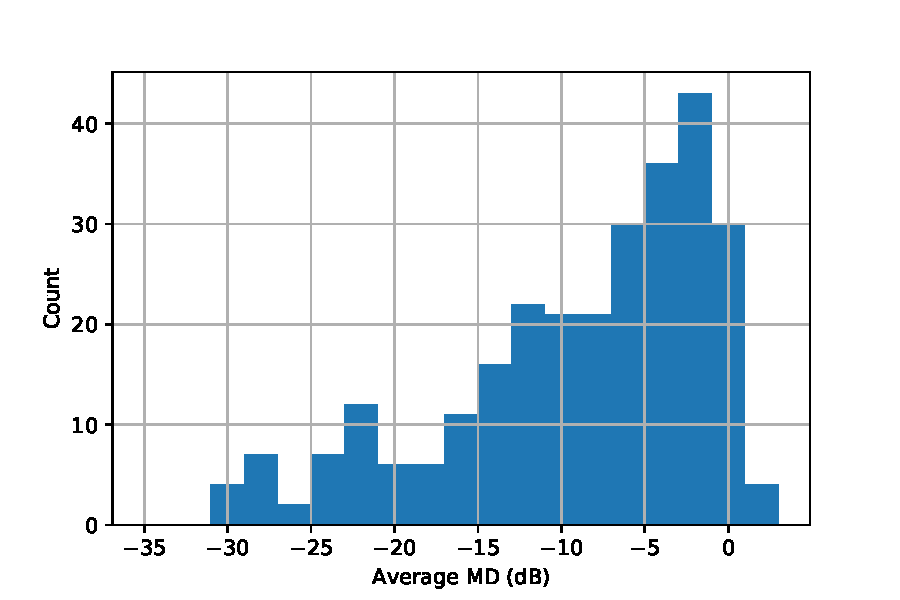
\includegraphics[width=0.6\textwidth]{mean_md_hist}	\caption{Distribution of eyes' average MD values within the Rotterdam dataset ($n=278$)}
%	\label{fig:mean_md_hist}
%\end{figure}

\subsection{Data Characteristics}

To investigate the composition of healthy versus glaucomatous patients the dataset, the characteristic of MD values in the dataset is investigated. In figure \ref{fig:mean_md_hist} the distribution of average MD value calculated from all tests administers on an eye for each of the $278$ eyes is shown. The mean and median of the distribution are $-8.9$ and $-6.8$ dB respectively. The data set contains mostly eyes with mild to moderate reduced MD values ($75\%$ of eyes have average MD $>-13.2$ dB).

To investigate the progression rate in the sample, an \ac{OLSLR} regression line is fit to each eye's MD history. The distribution of the slope (db/year) is shown in \ref{fig:mdpy_hist}


\begin{figure}[p]
	\centering
	\begin{subfigure}[b]{0.49\textwidth}
		\centering
		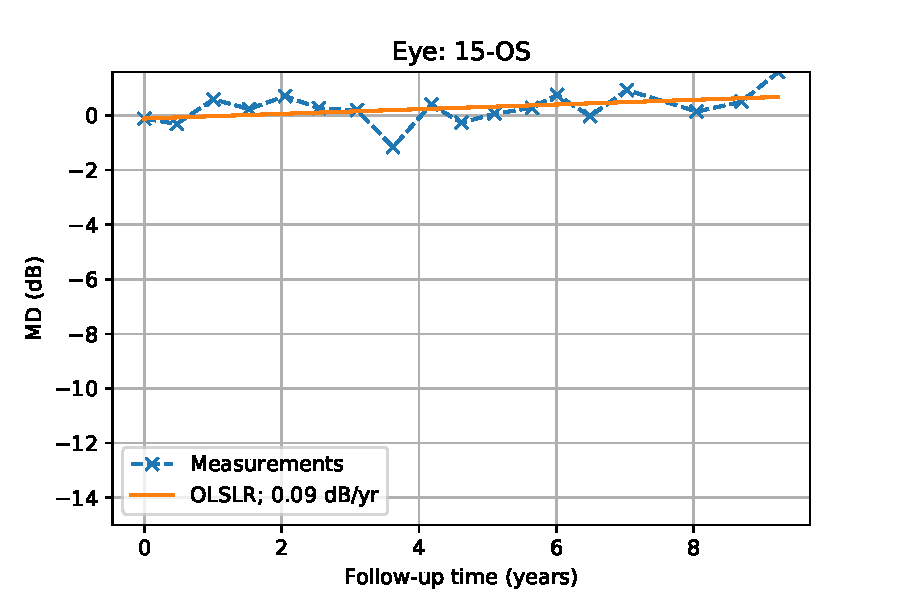
\includegraphics[width=\textwidth]{md_linear/15-OS}
		\caption{A stable healthy eye}
	\end{subfigure}
	\hfill
	\begin{subfigure}[b]{0.49\textwidth}
		\centering
		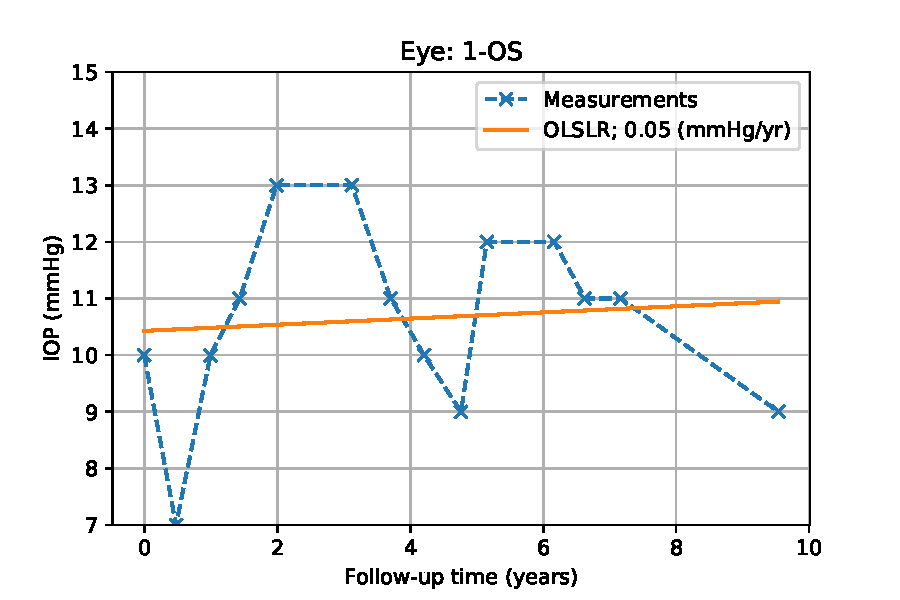
\includegraphics[width=\textwidth]{md_linear/1-OS}
		\caption{A depressed but stable eye}
	\end{subfigure}
	\hfill
	\begin{subfigure}[b]{0.49\textwidth}
	\centering
	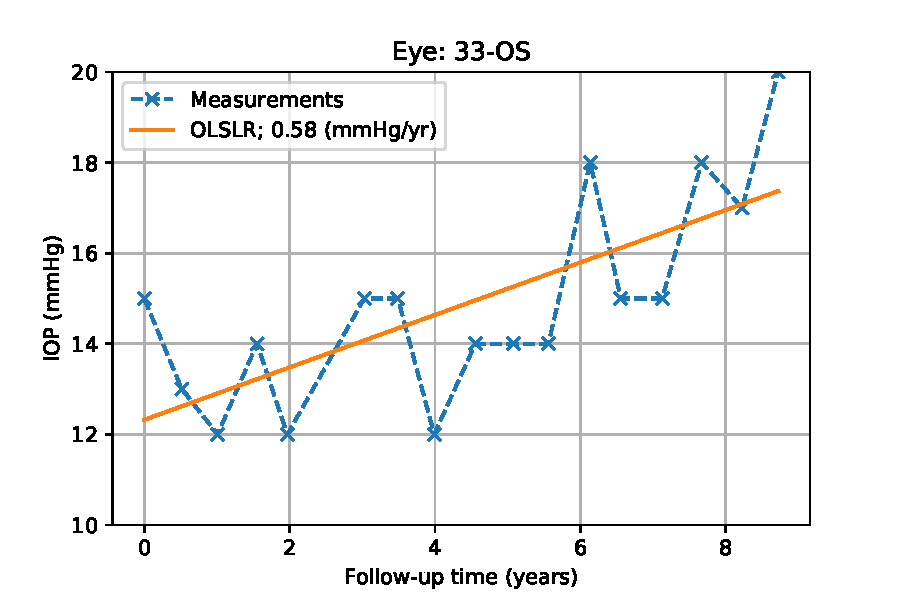
\includegraphics[width=\textwidth]{md_linear/33-OS}
	\caption{A moderately progressing eye}
	\end{subfigure}
	\hfill
	\begin{subfigure}[b]{0.49\textwidth}
	\centering
	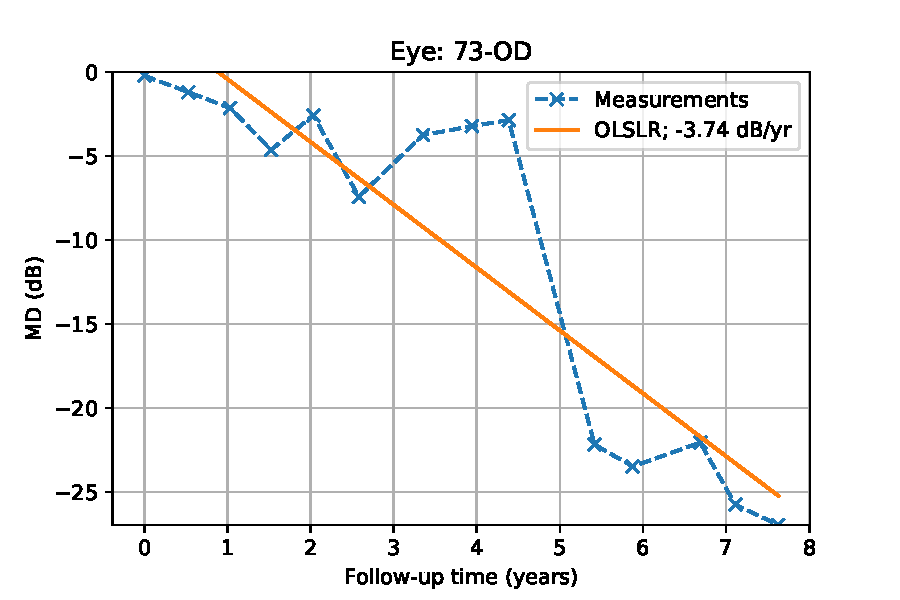
\includegraphics[width=\textwidth]{md_linear/73-OD}
	\caption{A suddenly rapidly progressing eye}
	\end{subfigure}
	\hfill
	\begin{subfigure}[b]{0.49\textwidth}
		\centering
		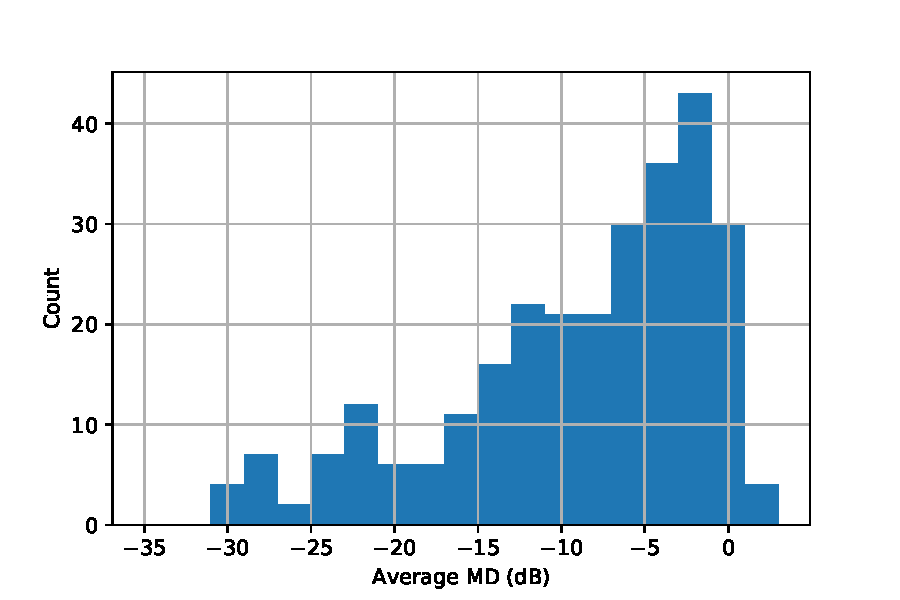
\includegraphics[width=\textwidth]{mean_md_hist}
		\caption{Mean MD}
	\end{subfigure}
	\hfill
	\begin{subfigure}[b]{0.49\textwidth}
		\centering
		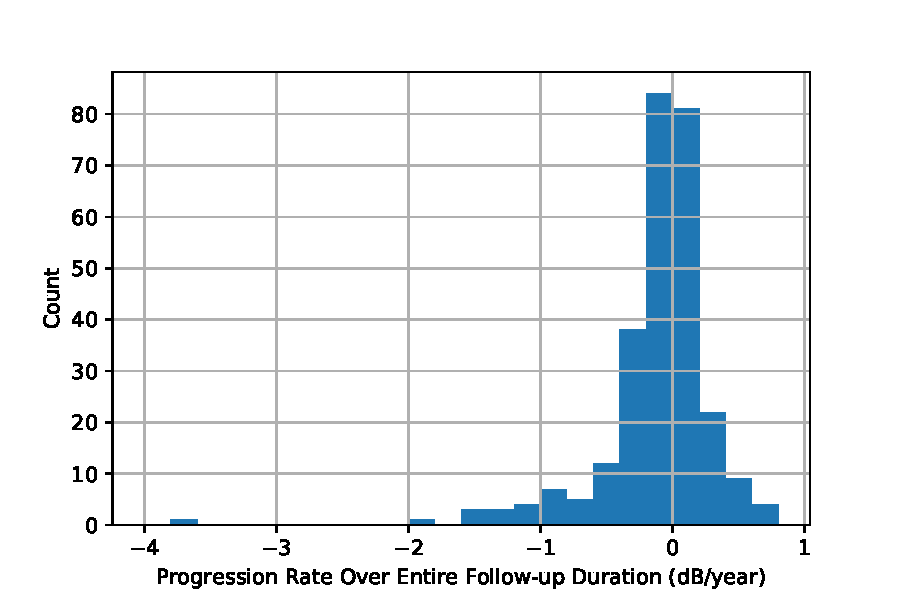
\includegraphics[width=\textwidth]{mdpy_hist}
		\caption{Progression rate $\Delta$MD/yr}
	\end{subfigure}
	\caption{Overview of the Rotterdam Longitudinal Glaucomatous \ac{VF} Dataset. (a-d) Select examples of the longitudinal \ac{VF} test results. (e) Distribution of mean MD value over each eye's follow-up duration. A lower mean MD value represents a more depressed eye and likely indicates more severe disease. Not that since perimeters typically have a dynamic range of $0$--$34$ dB, an MD of $-30$ essentially indicates a blind/almost blind eye. (f) Distribution of progression rate of each eye over the follow-up duration as measured by the rate of change of MD. (e-f) shows that a large number of eyes are relatively healthy and most eyes did not progress. This is likely due to either the slowly progressing nature of the glaucoma disease or due to appropriate intervention by clinicians.}
% 	\label{fig:study_site}
\end{figure}




